%----------------------------------------------------------------------------------------
\chapter{Monte-Carlo methods}
\label{sec:monte:carlo}
\index{Monte Carlo Method}
%----------------------------------------------------------------------------------------
Monte Carlo methods are computational algorithms which rely on repeated random sampling to obtain numerical results. The principle is to use randomness to solve the problem because it is difficult or impossible to utilize other approaches. A fun fact is that when the Monte Carlo Method was developed in the 1940s by Ulam and von Neumann they called the method Monte Carlo which refers to the Monte Carlo Casino in Monaco where Ulam's uncle gambled. Today Monte Carlo methods are widely used in following three problem classes:
\begin{itemize}
\item Optimization,
\item Numerical integration, and
\item Probability distributions.
\end{itemize}
For the importance of the method we refer to~\cite{kroese2014monte} and for more details about Monte Carlo Methods, we refer to~\cite{shonkwiler2009explorations}.\\

Let us look into the computational aspects of the Monte Carlo methods. Independent on the problem class a general pattern is observed
\begin{enumerate}
\item Define the input parameters,
\item Randomly chose input parameters,
\item Do deterministic computations on the inputs,
\item Aggregate the results\text{.}
\end{enumerate}

\begin{figure}[h]
  \begin{center}
  \begin{tikzpicture}
\draw (0,0) -- (2,0) -- (2,2) -- (0,2) -- cycle;
\draw[fill=cadetgrey, opacity=0.5] (1,1) circle (1cm);
\draw[->] (1,1) -- (2,1);
\draw[fill=black] (1,1) circle (0.05cm);
\node[above] at (1.5,1) {\small $r=\sfrac{1}{2}$};
\draw[<->] (0,-0.35) -- (2,-0.35);
\node[below] at (1,-0.35) {\small $1$};
\draw[<->] (-0.35,0) -- (-0.35,2);
\node[left] at (-0.35,1) {\small $1$};
\end{tikzpicture}
  \end{center}
  \caption{Sketch of the geometry used within the Monte Carlo method to estimate the number $\pi$.}
  \label{fig:monte}
\end{figure}
To understand these for steps, we will compute the value of $\pi$ using a Monte Carlo method. Note that this example is just for educational purposes. Figure~\ref{fig:monte} sketches the two ingredient a unit square and a circle needed to estimate $\pi$. First, a unit square $1 \times 1$ which means both sides have the length of one is drawn. The area $A_s$ is one, since we have a unit square. Second, a circle with the radius of $r=\sfrac{1}{2}$ is drawn at the center of the unit square. The area of the circle is $A_c=\pi r^2$. Using the radius $r=\sfrac{1}{2}$ the area is $A_c=\pi(\sfrac{1}{2})^2=\sfrac{\pi}{4}$. Now, since we have defined the area of the circle and the square, we can use them to estimate the value of $\pi$ by
\begin{align}
A_c &= \sfrac{\pi}{4} \notag\\
\pi &= 4 A_c \notag\\
\pi &= 4 \sfrac{A_c}{A_s}\text{.}
\end{align}
Note that the going from the first equation to the second one is just a multiplication by four. Going from the second line to the third line, we use the fact that the area of the square is one. \\

Now, we can estimate $\pi$ by the general pattern described above
\begin{itemize}
\item \textbf{Define the input parameters}: \\ A coordinate  $(x,y)\in\mathbb{R}$ in the domain of the unit square $[0,1]\times [0,1]$
\item\textbf{ Randomly chose input parameters}:\\ We randomly draw values for $x$ and $y$ in the range of $[0,1]$ for $N$ times
\item \textbf{Do deterministic computations on the inputs}:  \\
we have to validate if the coordinate $(x,y)$ is inside the circle or not by do the computation $x^2+y^2\leq 1$. If the coordinate is inside the circle we increment $N_C$.
\item \textbf{Aggregate the results}: \\
We compute $\pi\approx \sfrac{4N_c}{N}$
\end{itemize}
\vspace{0.25cm}

Figure~\ref{fig:algorithm:monte} shows the flow chart of the algorithm for estimating $\pi$ using the Monte Carlo method. First, the decision if the current draw of the random number is less than the total amount of random numbers $N$. If we have not draw enough random numbers, we have to guess to two random numbers $x$ and $y$, see Section~\ref{sec:random:numbers} for how to generate random numbers in C++. Next, we have to check if the drawn coordinate $(x,y)$ is within the circle and update the number of points within the circle $N_c$. We have to repeat this tasks until $i>N$. If we have drawn enough random number, we can compute $\pi\approx\sfrac{4N_c}{N}$ and finish the program.\\

\begin{figure}[tb]
    \centering
	\begin{tikzpicture}[node distance=1.125cm, scale=0.75, transform shape]
	\node (start) [startstop] {Start}; 
	\node (dec1) [decision, below of=start , yshift=-1.cm] { $i < N$};
	\node (n0) [process, below of=dec1,yshift=-1.cm] {Draw random number $x$ and $y$};
	\node (dec2) [decision, below of=n0 , yshift=-1.cm] { $x^2 + y^2 < 1$};
	\node (n1) [process, below of=dec2,yshift=-1.cm] {Increment $N_C$};
	\node (n2) [process, below of=n1,yshift=-1.cm] {Increment $i$};
	\node (n2) [process, below of=n1,yshift=-1.cm] {Increment $i$};
	\node (n3) [process, right of=dec1,xshift=2.5cm] {Compute $\sfrac{4N_c}{N}$};
	\node (stop) [startstop, right of=dec1, xshift=6.cm] {Finished}; 
	%lines
	\draw [->] (start) -- (dec1);
	\draw [->] (dec1) -- (n0);
	\draw [->] (n0) -- (dec2);
	\draw [->] (n1) -- (n2);
	\draw [->] (n3) -- (stop);
	%dec1
	\draw [->] (dec1) -- node[anchor=north] {no} (n3);
	\draw [->] (dec1) -- node[anchor=west] {yes} (n0);	
	\draw [->] (dec2) -- node[anchor=west] {yes} (n1);	
	\draw [->] (n2.west) -- ++(-3.0,0) -- ++(0,8.5) -- ++(3.5,0);
	\draw [->] (dec2)  -- ++(-4.5,0) ;
	\end{tikzpicture}
	\caption{Flow chart for the Monte Carlo method to estimate $\pi$.}
	\label{fig:algorithm:monte}
\end{figure}

Next, we can ask the question what is a good choice for $N$ to get a good approximation of $pi$. Figure~\ref{fig:monte:carlo:samples} shows the distribution of the point inside the circle (\textcolor{amaranth}{red}) and outside of the circle (\textcolor{azure}{blue}) for $N=10$, $N=100$, and $N=1000$ random numbers. One can see that a certain amount of random numbers is needed to have enough samples inside and outside of the circle. Figure~\ref{fig:monte:carlo} shows the absolute error in percent for various amount of random numbers. One can see that with thousand random numbers the accuracy is quite reasonable. 


\begin{figure}[bt]
\begin{subfigure}{.3\textwidth}
  \centering
\def\x{0}
\def\y{0}
\def\k{0}
\def\radius{4}
\begin{tikzpicture}
    \draw[fill=cadetgrey, opacity=0.1] (\radius,0) arc(0:90:\radius) -- (0,0) -- cycle;
    \draw[gray, opacity=0.25] (0,0) rectangle (\radius,\radius);
    \draw[->] (0,0) -- (1.1*\radius,0);
    \draw[->] (0,0) -- (0,1.1*\radius);
    \foreach \i in {1,2,...,10}{%
        \pgfmathsetmacro\x{\radius*rnd}%
        \pgfmathsetmacro\y{\radius*rnd}%
        \pgfmathsetmacro\k{(pow(\x,2)+pow(\y,2)) <pow(\radius,2)}%
        \pgfmathparse{ifthenelse(\k==1,"amaranth","azure")}%
        \fill[\pgfmathresult] (\x,\y)circle(0.75pt);%
    }
\end{tikzpicture}
  \caption{$N=10$}
  \label{fig:sub-first}
\end{subfigure}
\hfill
\begin{subfigure}{.3\textwidth}
  \centering
\def\x{0}
\def\y{0}
\def\k{0}
\def\radius{4}
\begin{tikzpicture}
    \draw[fill=cadetgrey, opacity=0.1] (\radius,0) arc(0:90:\radius) -- (0,0) -- cycle;
    \draw[gray, opacity=0.25] (0,0) rectangle (\radius,\radius);
    \draw[->] (0,0) -- (1.1*\radius,0);
    \draw[->] (0,0) -- (0,1.1*\radius);
    \foreach \i in {1,2,...,100}{%
        \pgfmathsetmacro\x{\radius*rnd}%
        \pgfmathsetmacro\y{\radius*rnd}%
        \pgfmathsetmacro\k{(pow(\x,2)+pow(\y,2)) <pow(\radius,2)}%
        \pgfmathparse{ifthenelse(\k==1,"amaranth","azure")}%
        \fill[\pgfmathresult] (\x,\y)circle(0.75pt);%
    }
\end{tikzpicture}
  \caption{$N=100$}
\end{subfigure}
\hfill
\begin{subfigure}{.3\textwidth}
  \centering
\def\x{0}
\def\y{0}
\def\k{0}
\def\radius{4}
\begin{tikzpicture}
    \draw[fill=cadetgrey, opacity=0.1] (\radius,0) arc(0:90:\radius) -- (0,0) -- cycle;
    \draw[gray, opacity=0.25] (0,0) rectangle (\radius,\radius);
    \draw[->] (0,0) -- (1.1*\radius,0);
    \draw[->] (0,0) -- (0,1.1*\radius);
    \foreach \i in {1,2,...,1000}{%
        \pgfmathsetmacro\x{\radius*rnd}%
        \pgfmathsetmacro\y{\radius*rnd}%
        \pgfmathsetmacro\k{(pow(\x,2)+pow(\y,2)) <pow(\radius,2)}%
        \pgfmathparse{ifthenelse(\k==1,"amaranth","azure")}%
        \fill[\pgfmathresult] (\x,\y)circle(0.75pt);%
    }
\end{tikzpicture}
  \caption{$N=1000$}
  \label{fig:sub-second}
\end{subfigure}
\caption{Distribution of the point inside the circle (\textcolor{amaranth}{red}) and outside of the circle (\textcolor{azure}{blue}) for $N=10$, $N=100$, and $N=1000$ random numbers.}
\label{fig:monte:carlo:samples}
% This example was adapted from https://tex.stackexchange.com/questions/244488/monte-carlo-method-drawing
\end{figure}


\begin{figure}[tb]
\centering
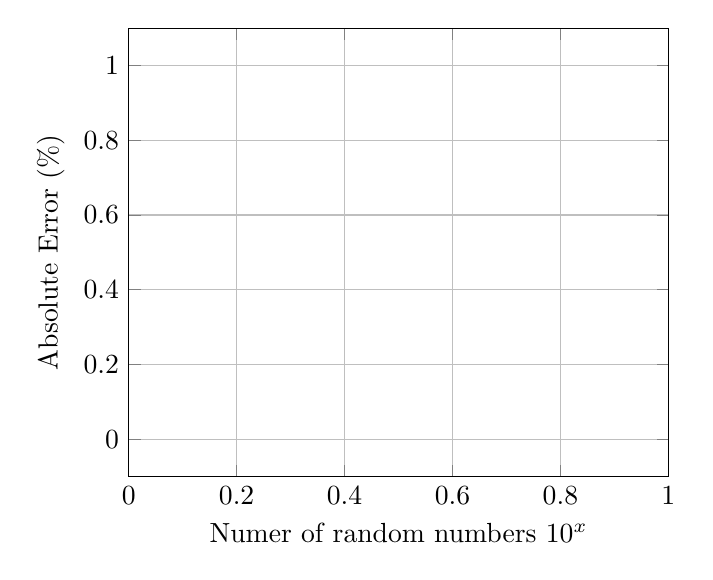
\begin{tikzpicture}
\begin{axis}
[
	xmin=0,   xmax=4,
	grid=major,
	xlabel=Numer of random numbers $10^x$,
	ylabel=Absolute Error (\%)
]
\montecarlo{10}{1}
\montecarlo{100}{2}
\montecarlo{1000}{3}
\end{axis}
\end{tikzpicture}
\caption{The absolute error in percent for various amount of random numbers. One can see that with thousand random numbers the accuracy is quite reasonable. }
\label{fig:monte:carlo}
\end{figure}

\begin{exercise}
Make a list of which C++ features we need to implement the flow chart in Figure~\ref{fig:algorithm:monte}.
\end{exercise}

\begin{exercise}
Implement the Algorithm in Figure~\ref{fig:algorithm:monte} using the random numbers in Section~\ref{sec:random:numbers}.
\end{exercise}


%----------------------------------------------------------------------------------------
\chapter{$N$-body problems}
\index{$N$-body problems}
\label{sec:nbody}
%----------------------------------------------------------------------------------------
The $N$-body problem is the physically problem of predicting the individual motions of a group of celestial objects interacting with each others gravitationally. In laymen terms we want to predict the interactive forces and the motion of all celestial bodies in all future times. We assume that the know their orbital properties, \emph{e.g.}\ the initial positions, velocity, and time.\\

Before we look into the $N$-body problem, we stepping back and look into the two-body problem. Let us look at two gravitational bodies with the massed $m_i$ and $m_j$ and their positions $\mathbf{r}_i,\mathbf{r}_j\in\mathbb{R}^3$. To define the equation of motion, we have to look in the following definitions:
\vspace{0.25cm}
\begin{enumerate}
\item \textbf{The Law of Gravitation}: \\
The force of $m_i$ acting on $m_j$ is 
\begin{align}
\mathbf{F}_{ij}= G m_i m_j \frac{\mathbf{r}_j-\mathbf{r}_2}{\vert \mathbf{r}_1-\mathbf{r}_i \vert^3}\text{,}
\end{align}
see Figure~\ref{fig:nbody:motion}. The universal constant of gravitation $G$ was estimated as $6.67408\cdot 10^{-11}m^3kg^{-1}s^{-2}$ in 2014~\cite{mohr2016codata}.
\item \textbf{Velocity and acceleration}: 
\begin{enumerate}
\item The velocity of $m_i$ reads as
\begin{align}
\mathbf{v}_i = \frac{d \mathbf{r}_i}{dt} \label{eq:nbody:vel}
\end{align}
\item The acceleration of $m_i$ reads as
\begin{align}
\mathbf{a}_i = \frac{d \mathbf{v}_i}{dt} \label{eq:nbody:acc}
\end{align}
\end{enumerate}
For more details about vector and basic vector operations, we refer to Section~\ref{sec:linalg:vectors}.
\item \textbf{The second Law of Mechanics}:  (Force is equal mass times acceleration) 
\begin{align}
\mathbf{F}= m \mathbf{a} \label{eq:law:first}
\end{align}
\end{enumerate}
With these three definitions, we can derive the equation of motion for the first body as follows
\begin{align}
\mathbf{F}_{ij}&=G m_i m_j \frac{\mathbf{r}_j-\mathbf{r}_i}{\vert \mathbf{r}_j-\mathbf{r}_i \vert^3} \label{eq:nbody:motion1} \\
m_i \mathbf{a}_i &= G m_i m_j \frac{\mathbf{r}_j-\mathbf{r}_i}{\vert \mathbf{r}_i-\mathbf{r}_j \vert^3} \label{eq:nbody:motion2} \\
\frac{d \mathbf{v}_i}{dt} & = G m_j \frac{\mathbf{r}_j-\mathbf{r}_i}{\vert \mathbf{r}_j-\mathbf{r}_i \vert^3} \label{eq:nbody:motion3} \\
\frac{d^2 \mathbf{r}_i}{dt^2} & = G m_j \frac{\mathbf{r}_j-\mathbf{r}_i}{\vert \mathbf{r}_j-\mathbf{r}_i \vert^3}
\label{eq:nbody:motion4}
\end{align}
To get from Equation~\eqref{eq:nbody:motion1} to Equation~\eqref{eq:nbody:motion2}, we substitute $\mathbf{F}_{ij}$ by $m_i \mathbf{a}_i$ using Equation~\ref{eq:law:first}.  From Equation~\eqref{eq:nbody:motion2} to Equation~\eqref{eq:nbody:motion3}, we divide by $m_i$ and substitute $\mathbf{a}_i$ by Equation~\ref{eq:nbody:acc}. From Equation~\eqref{eq:nbody:motion3} to From Equation~\eqref{eq:nbody:motion4}, we substitute Equation~\ref{eq:nbody:vel}. Note that we used Newton's law of universal gravitation~\cite{newton1833philosophiae}.\\


\begin{figure}[tb]
\centering
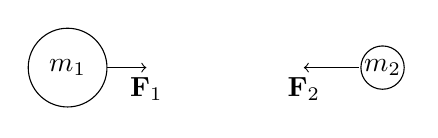
\begin{tikzpicture}
\draw (-2,0) circle (0.5cm);
\draw (2,0) circle (0.275cm);
\node at (-2,0) {$m_1$};
\node at (2,0) {$m_2$};
\draw[->] (-1.5,0)--(-1,0);
\draw[->] (1.7,0)--(1,0);
\node[below] at (-1,0) {$\mathbf{F}_1$};
\node[below] at (1,0) {$\mathbf{F}_2$};
\end{tikzpicture}
\caption{Sketch of the two celestial bodies with the masses $m_1$ and $m_2$ and the gravitational interaction forces $\mathbf{F}_1$ and $\mathbf{F}_1$. Equation~\ref{eq:nbody:motion4} shows the equation of motion for the two-body system.   }
\label{fig:nbody:motion}
\end{figure}

Now, we formulate the problem for $n$ bodies assuming that the force at one body is equal to the sum over all bodies, except the body itself
\begin{align}
\mathbf{F}_i = \sum\limits_{j=1,i\neq j}^n \mathbf{F}_{ij} = \sum\limits_{j=1,,i\neq j}^n G  m_j \frac{\mathbf{r}_j - \mathbf{r}_i}{\vert \mathbf{r}_j - \mathbf{r}_i\vert^3} \text{.} \label{eq:nbody:motion}
\end{align}
These are the laws of conservation for the $N$-body problem:
\begin{enumerate}
\item Linear Momentum: $\sum\limits_{i=1}^n m_i \mathbf{v}_i = M_0$
\item Center of Mass: $\sum\limits_{i=1}^n m_i \mathbf{r}_i = M_0 t + M_1$
\item Angular Momentum: $\sum\limits_{i=1}^n m_i (\mathbf{r}_i \times \mathbf{v}_i) = \mathbf{c}$
\item Energy: T-U=h with \\
$ T = \frac{1}{2} \sum\limits_{i=1}^n m_i \mathbf{v}_i \circ \mathbf{v}_i  , U= \sum\limits_{i=1}^n \sum\limits_{j=1}^n G \frac{m_i m_j}{\vert\mathbf{r}_i - \mathbf{r}_j\vert} $
\end{enumerate}
Note that these laws are just shown for completeness. For more details about the theory and the derivations, we refer to~\cite{aarseth2008cambridge,aarseth2003gravitational}. This book focuses on the implementation details and just provides the basics to implement the $N$-body problem within C++.

%----------------------------------------------------------------------------------------
\section{Algorithm}
%----------------------------------------------------------------------------------------
Figure~\ref{fig:nbody:algorithm} shows the three steps for the $N$-body simulation. In this section, we focus on the implementation details of the first two steps. Equation~\ref{eq:nbody:motion} shows how to compute the force for one celestial object. Recall, that the $\sum$ translate to a \cpp{for} loop as we discussed in Section~\ref{sec:iteration:statements}. To compute the forces of all bodies, the so-called nested \cpp{for} loop or direct sum is utilized. Listing~\ref{code:directsum} shows the concept of the direct sum which is robust, accurate, and completely general. However, the computational costs per body are $\mathcal{O}(n)$ and the computational costs for all bodies are $\mathcal{O}(n^2)$. The symbol $\mathcal{O}$ is the so-called Big O notation which is used for algorithms to describe how their run time or space space requirements grow as the input size grows. In our case the computational costs per body increase linear, since we have to compute the force $n-1$ times for all particles. The Big O notation $\mathcal{O}(n)$ means that the total amount of computational costs in less or equal $n$. These symbols are defined in the Bachmann–Landau notation\index{Bachmann–Landau notation}~\cite{bachmann1894analytische,landau2000handbuch,knuth1997art}. For all bodies the computational cost increases two the power of two since we have to compute the forces $n-1$ times for all all $n$ bodies. For small amount of celestial objects the direct sum is feasible, however, for larger amounts the tree-based codes or the Barnes-Hut method~\cite{barnes1986hierarchical} reduce the computational costs to $\mathcal{O}(n\log(n))$. \\

\begin{figure}[tb]
\centering
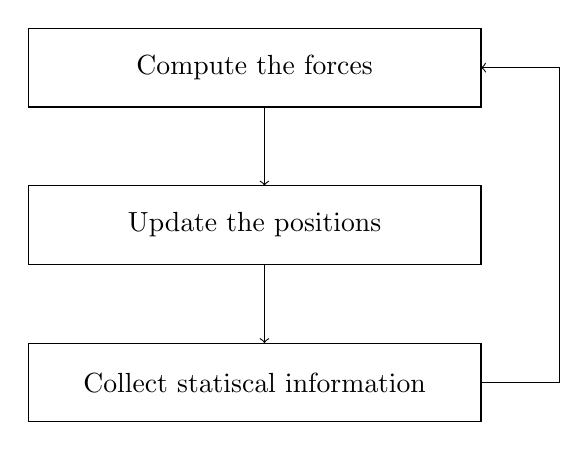
\begin{tikzpicture}
\draw (-3.75,0) rectangle (2,1) node[pos=.5] {Compute the forces};
\draw[->](-0.75,0) -- (-0.75,-1);
\draw (-3.75,-2) rectangle (2,-1) node[pos=.5] {Update the positions};
\draw[->](-0.75,-2) -- (-0.75,-3);
\draw (-3.75,-4) rectangle (2,-3) node[pos=.5] {Collect statiscal information};
\draw[->] (2,-3.5) -- (3,-3.5) -- (3,0.5) -- (2,0.5);
\end{tikzpicture}
\caption{The three steps of the algorithm for the $N$-body simulation. First, the forces for all objects are computed using Equation~\ref{eq:nbody:motion}. Second, the updated positions are computed using Equation~\ref{eq:position:update} and Equation~\ref{eq:position:update}. Third, the statistical information is evaluated.  }
\label{fig:nbody:algorithm}
\end{figure}


\begin{lstlisting}[language=c++,caption={Example for the so-called direct sum\index{direct sum}.\label{code:directsum}},float,floatplacement=tb]
for(size_t i = 0; i < bodies.size(); i++)
	for(size_t j = 0; j < bodies.size(); j++)
		if ( i != j )
			//Compute forces
\end{lstlisting}

For the second step of the algorithm, we need to update the positions for the evolution of the system over the time $T$. For the discretization in time, we define following quantities:
\begin{itemize}
\item $\Delta t$ the uniform time step size
\item $t_0$ the beginning of the evolution
\item $T$ the final time of the evolution
\item $k$ the time steps such that $k\Delta t=T$.
\end{itemize}
Next, we need to compute the derivatives to obtain the velocity and the acceleration of each celestial object. One numerical method to approximate the derivation is given by
\begin{align}
u'(x) \approx \frac{u(x+h)-u(x)}{h}
\end{align}
which is the s-called finite difference method. Figure~\ref{fig:nbody:finitedifference} sketches the principle of the finite difference method. For a sufficient small enough $h$, we can approximate the derivation at the coordinate $x$. For example choosing $h=1$ and $x=3$, we get $u'(x)=\sfrac{(4-3)}{1}=1$ which confirms with $u'(x)=1$ using the analytic derivation of $u(x)$. Now we can use Euler method to compute the updated positions at time $t_{k+1}$. First, we approximate the velocity using the finite difference scheme
\begin{align}
\mathbf{v}_i(t_k) = \frac{d\mathbf{r}_i}{dt} \approx \frac{\mathbf{r}_i(t_{k+1})-\mathbf{r}_i(t_k)}{\Delta t}\label{eq:vel}\text{.}
\end{align}
We do the same for the acceleration
\begin{align}
\mathbf{a}_i(t_k) = \frac{d\mathbf{v}_i}{dt}   \approx  \frac{\mathbf{v}_i(t_k)-\mathbf{v}_i(t_k-1)}{\Delta t} = \frac{\mathbf{F}_i}{m_i}  \label{eq:acc} 
\end{align}
from Equation~\ref{eq:law:first} we get $\mathbf{a}_i=\sfrac{\mathbf{F}_i}{m_i}$. More details~\cite{strikwerda2004finite,leveque2007finite,euler1824institutionum}. With the above approximations the velocity is computed as
\begin{align}
\mathbf{v}_i(t_k) = \mathbf{v}_i(t_{k-1}) + \Delta t \frac{\mathbf{F}_i}{m_i} \label{eq:position:update}
\end{align}
using Equation~\eqref{eq:acc} and the fact that the finite difference approximation of the acceleration is equal to $\sfrac{\mathbf{F}_i}{m_i}$. Finally, the updated position is computed as
\begin{align}
\mathbf{r}_i(t_{k+1}) = \mathbf{r}_{t_k} + \Delta t \mathbf{v}_i(t_k)  \label{eq:position:update}
\end{align} 
using Equation~\eqref{eq:vel}. Note that we used easy methods to update the positions and more sophisticated methods, \emph{e.g.}\ Crank--Nicolson method~\cite{crank1947practical}, are available

\begin{exercise}
Look into the equations in this section and try to derive the Equation~\ref{eq:position:update} and Equation~\ref{eq:position:update} on your own.
\end{exercise}

\begin{exercise}
Implement the $N$-body problem using the template code\link{https://github.com/diehlpkteaching/N-Body} on GitHub.
\end{exercise}

\begin{figure}[tb]
\centering
\begin{tikzpicture}
\begin{axis}[
        xmin=0, xmax=6, % x scale
        ymin=0, ymax=6, % y scale
]
\addplot[azure,thick]    {x};
\legend{$u(x)$}
\addplot[amaranth, mark=*] coordinates{(3,3)} node[midway,above left,amaranth] {$u(x)$};
\addplot[amaranth,  mark=*] coordinates{(4,4)} node[midway,above left,amaranth] {$u(x+h)$};
\addplot +[mark=none,cadetgrey] coordinates {(3, 3) (4, 3)};
\addplot +[mark=none,cadetgrey] coordinates {(4, 3) (4, 4)};
\addplot[cadetgrey,  mark=none] coordinates{(3.5,3)} node[midway,below] {$h$};
\end{axis}
\end{tikzpicture}
\caption{The principle of the finite difference method. For a sufficient small enough $h$, we can approximate the derivation at the coordinate $x$. For example choosing $h=1$ and $x=3$, we get $u'(x)=\sfrac{(4-3)}{1}=1$ which confirms with $u'(x)=1$ using the analytic derivation of $u(x)$. Now we can use Euler method to compute the updated positions at time $t_{k+1}$.}
\label{fig:nbody:finitedifference}
\end{figure}

%----------------------------------------------------------------------------------------
\chapter{Peridynamics}
\label{sec:pd}
%----------------------------------------------------------------------------------------
Peridynamic, a alternative formulation of continuum mechanics with a focus on discontinuous displacement as they arise in fracture mechanics, was introduced by Silling in 2000~\cite{silling2000reformulation,silling2005meshfree}. Models crack and fractures on a mesoscopic scale using Newton's second law (force equals mass times acceleration)
\begin{align}
F = m \cdot a = m \cdot \ddot X \text{.}
\end{align}



%----------------------------------------------------------------------------------------
\section{Brief introduction in classical continuum mechanics}
%----------------------------------------------------------------------------------------
We briefly look into the ingredients of classical continuum mechanics which are needed to introduce peridynamics. In Figure~\ref{fig::chapter2:01} on the lift-hand side, we see the continuum in the reference configuration $\Omega_0 \subset \R^3$ which is the state where we have no internal forces and we are in the equilibrium. We denote these positions with capitalized $X \in \R^3$ to distinguished with the new position after the deformation $\phi : \Omega_0 \rightarrow \R^3$. The deformation implied for example by some external forces moves the continuum from the reference configuration  $\Omega_0$ to the current configuration $\Omega(t)$. The new position of $X$ is now $x(t,X)$.\\

Let us look more closely in the definitions above. The deformation $\phi:[0,T]\times\R^3\rightarrow\R^3$ of a material point $X$ in the reference configuration $\Omega_0$ to the so-called current configuration $\Omega(t)$ is given by
\begin{align*}
\phi(t,X) := id(X) + u(t,X) = x(t,X) \text{,}
\end{align*}
where $u:[0,T]\times\R^3\rightarrow\R^3$ refers to the displacement
\begin{align*}
u(t,X):= x(t,X) - X\,\text{.}
\end{align*}
The stretch $s:[0,T]\times\R^3\times\R^3\rightarrow\R^3$ between the material point $X$ and the material point $X'$ after the deformation $\phi$ in the configuration $\Omega(t)$ is defined by
\begin{align*}
s(t,X,X') := \phi(t,X') - \phi(t,X) \,\text{.}
\end{align*}
We just covered the prerequisites of classical continuum mechanics which are necessary to introduce the peridynamic theory. For more details, we refer to~\cite{gurtin1982introduction,liu2013continuum}.

\begin{figure}[tb]
\centering
\begin{tikzpicture}
\draw[fill=blue, opacity=0.5](1,1) circle (1);
 \node at (1,2.35) {{\small $\Omega_0$}};
 \draw[fill=blue,](1,1) circle (0.075);
 \node at (1,0.725) {{\small $X$}};
 \node at (6,1) {
\includegraphics[scale=1.25]{images/deformation.pdf}};
 \node at (6,2.35) {{\small $\Omega(t)$}};
 \draw[fill=blue,](6,0.725) circle (0.075);
 \node at (6,0.45) {{\small $x(t,X)$}};
 \node at (3.75,2.45) {{\small $\phi:\Omega_0\rightarrow \R^3$}};
 \draw [arrow, bend angle=45, bend left] (1.95,1.25) to (5.8,1);
\end{tikzpicture}
\caption[The continuum in the reference configuration $\Omega_0$ and after the deformation $\phi : \Omega_0 \rightarrow \R^3$ in the current configuration $\Omega(t)$ at time $t$.]{The continuum in the reference configuration $\Omega_0$ and after the deformation $\phi : \Omega_0 \rightarrow \R^3$ with $\det(\text{grad}\;\phi) > 0$ in the current configuration $\Omega(t)$ at time $t$.}
\label{fig::chapter2:01}
\end{figure}

%----------------------------------------------------------------------------------------
\section{Brief introduction in bond-based peridynamics}
%----------------------------------------------------------------------------------------
We can use Newton;s second law (force equals mass times acceleration) and formulate it as
\begin{align}
\rho(X)a(t,X):=
\int\limits_{B_\delta(X)} f\left(t,x(t,X')-x(t,X), X'-X\right)dX' + b(t,X)\,\text{,}
\label{eq::chapter2:01}
\end{align}
to compute the acceleration $a:\ftime\times\R^3\rightarrow\R^3$ of a material point at position $X$ at time $t$. With the pair-wise force function $f:[0,T]\times\R^3\times\R^3\rightarrow\R^3$, the mass density $\rho(X)$, and the external force $b:[0,T]\times\mathbb{R}^3\rightarrow\mathbb{R}^3$. Following assumptions are made
\begin{enumerate}
\item The medium is continuous (equal to a continuous mass density field exists)
\item Internal forces are contact forces (equal to that material points only interact if they are separated by zero distance.
\item Conservation laws of mechanics apply
\begin{enumerate}
\item Conservation of mass
\item Conservation of linear momentum
\begin{align*}
f(t,-(x(t,X')-x(t,X)),-(X'-X))= -f(t,x(t,X')-x(t,X), X'-X)
\end{align*}
\item Conservation of angular momentum
\begin{align*}
(x(t,X')-x(t,X)+X'-X) \times f\left(t,x(t,X')-x(t,X), X'-X\right) = 0
\end{align*}
\end{enumerate}
\end{enumerate}

%----------------------------------------------------------------------------------------
\subsection{Material model}
%----------------------------------------------------------------------------------------
There are several material models available, however, we look into the Prototype Microelastic Brittle (PMB) model, since it was one of the first material models. In this model the assumption is made that the pair-wise force $f$ only depends on the relative normalized bond stretch $s:[0,T]\times\mathbb{R}^3\times\mathbb{R}^3\rightarrow\mathbb{R}$
\begin{align}
s(t,x(t,X')&-x(t,X),X'-X):= \\ &\frac{\vert\vert x(t,X')-x(t,X))\vert\vert - \vert\vert X'-X\vert\vert}{\vert\vert X'-X\vert\vert}\,\text{,} 
\end{align}
where $X'-X$ is the vector between the material points in the reference configuration $\Omega_0$ and $x(t,X')-x(t,X)$ is the vector between the material point in the current configuration $\Omega(t)$. As a material property, the so-called stiffness constant $\textcolor{azure}{c}$ is introduced and the pair-wise force function reads as
\begin{align}
f(t,x(t,X')-x(t,X),X'-X):=  \textcolor{blue}{c} \, s(t,x(t,X')-x(t,X),X'-X)\frac{x(t,X')-x(t,X)}{\Vert x(t,X')-x(t,X)\Vert} \text{.}
\end{align}
The pair-wise force function is shown in Figure~\ref{fig::force::sketch}. Which is a linear line with the slope \textcolor{azure}{blue}. Note that we do not have introduced damage to the material model yet. Therefore, a scalar valued history dependent function $\mu:[0,T]\times\mathbb{R}^3\times\mathbb{R}^3\rightarrow\mathbb{N}$ is added to the computation of the pair-wise force
\begin{align}
f(t,x(t,X')-x(t,X),X'-X)&:= \notag\\ & \textcolor{azure}{c} s(t,x(t,X')-x(t,X),X'-X) \notag\\&\mu\args \frac{x(t,X')-x(t,X)}{\Vert x(t,X')-x(t,X)\Vert}\,\text{.} 
\end{align}
with
\begin{align}
\mu(t,x(t,X')&-x(t,X),X'-X):= 
 \left\{
 \begin{aligned}
 & 1 \quad s(t,x(t,X')-x(t,X),X'-X) < \textcolor{azure}{s_{c}} \\
 %& \qquad -\alpha s_\text{smin}(t') \forall 0 \leq t' \leq t
%\\[1ex]
 & 0 \quad \text{otherwise}
\end{aligned}
 \right.
\end{align}
The pair-wise force function with the damage is incorporated is shown in Figure~\ref{fig::force::sketch::critical}.
With the scalar valued history dependent function $\mu$ the notion of damage $d(t,X):[0,T]\times\R^3\rightarrow\R$ can be introduced via
\begin{align}
d(t,X):= 1- \frac{\displaystyle\int\limits_{B_\delta(X)}\mu\args dX'}{\displaystyle\int\limits_{B_\delta(X)}dX'}\,\text{.}
\label{eq::damage:nodal}
\end{align}
To express damage in words, it is the ratio of the active (non-broken) bonds and the amount of bonds in the reference configuration within the neighborhood. Note that we have two material properties the stuffiness constant $\textcolor{blue}{c}$ and the critical stretch $\textcolor{blue}{s_c}$. We can related these to continuum mechanics as
\begin{align}
c = \frac{18K}{\pi\delta} \qquad \text{ and } \qquad s_c = \frac{5}{12} \sqrt{\frac{K_{Ic}}{K^2\delta}}
\end{align}
With $K$ is the bulk modulus and $K_Ic$ is the critical stress intensity factor.



\begin{figure}[bt]
\begin{subfigure}{.45\textwidth}
  \centering
\begin{tikzpicture}
 \begin{axis}[xlabel=$s$, axis lines=middle,ticks=none ,grid=major,ymax=0.75, ylabel=$f$]
 \addplot[domain=0:1,thick] {0.5 * x};
 \draw[gray,thick] (0.4,0.2) -- (0.6,0.2);
 \draw[gray,thick] (0.6,0.2) -- (0.6,0.3);
 \node at (0.525,0.225) {{\small \textcolor{azure}{$c$}}};
 \end{axis}
\end{tikzpicture}
\caption[Sketch of the pair-wise linear valued force function $f$ with the stiffness constant $c$ as slope.]{Sketch of the pair-wise linear valued force function $f$ with the stiffness constant \textcolor{azure}{$c$} as slope.}
\label{fig::force::sketch}
\end{subfigure}
\hfill
\begin{subfigure}{.45\textwidth}
  \centering
\begin{tikzpicture}
 \begin{axis}[xlabel=$s$, axis lines=middle ,grid=major,ymax=0.75, ylabel=$f$,xtick={1}, xticklabels={\textcolor{azure}{$s_c$}},yticklabels={,,}]
 \addplot[domain=0:1,thick] {0.5 * x};
 \addplot[domain=1:1.5,thick] {0 * x};
 \draw[gray,thick] (0.4,0.2) -- (0.6,0.2);
 \draw[gray,thick] (0.6,0.2) -- (0.6,0.3);
 \draw[gray,thick,dashed] (1,0) -- (1,0.5);
 \node at (0.525,0.225) {{\small \textcolor{azure}{$c$}}};
 \end{axis}
\end{tikzpicture}
\caption[Sketch of the pair-wise linear valued force function $f$ with the stiffness constant $c$ as slope and the critical bond stretch $s_c$.]{Sketch of the pair-wise linear valued force function $f$ with the stiffness constant \textcolor{azure}{$c$} as slope and the critical bond stretch \textcolor{azure}{$s_c$}.}
\label{fig::force::sketch::critical}
\end{subfigure}
\caption{}
% This example was adapted from https://tex.stackexchange.com/questions/244488/monte-carlo-method-drawing
\end{figure}

%----------------------------------------------------------------------------------------
\section{Discretization}
%----------------------------------------------------------------------------------------
To discretize the peridynamic equation of motion~\eqref{eq::chapter2:01}, the so-called EMU nodal discretization (EMU ND)~\cite{parks2008implementing} is used. All material points $X$ are placed at the nodes $\mathbf{X}:=\lbrace X_i \in \mathbb{R}^3\vert i=1,\ldots,n\rbrace$ of a regular grid in the reference configuration $\Omega_0$, see Figure~\ref{fig:emu}. We assume that the  discrete nodal spacing $\dx$ between $X_i$ and $X_j$ is defined as $\dx = \Vert X_j - X_i \Vert$ and is constant in all directions. For all material points at the nodes $\mathbf{X}:=\lbrace X_i \in \mathbb{R}^3\vert i=1,\ldots,n\rbrace$ a surrounding volume $\mathbf{V}:=\lbrace\ \mathbf{V}_i \in \mathbb{R}\vert i=1,\ldots,n\rbrace$ is assumed. These volumes are non overlapping $\mathbf{V}_i \cap \mathbf{V}_j = \emptyset$ and recover the volume of the volume of the reference configuration $\sum_{i=1}^n \mathbf{V}_i = \mathbf{V}_{\Omega_0}$. Using this assumptions the integral sign in the peridynamic equation of motion is replaced by a sum and reads as
\begin{align}
\rho(X_i)a(t,X_i)&=\sum\limits_{X_j\in B_\delta(X_i)}  f\left(t,x(t,X_j)-x(t,X_i), X_j-X_i\right)d\mathbf{V}_j + b(t,X_i) \text{.}
\end{align}
The discrete interaction zone $B_\delta(X_i)$ of $X_i$ is given by $B_\delta(X_i):=\lbrace X_j \vert \,\vert\vert X_j-X_i\vert\vert \leq \delta\rbrace$ which means that all the materials point within the circle in Figure~\ref{fig:emu} exchange pair-wise forces with the discrete material point $X_i$.\\

From the computational aspects, we have to store the discrete interaction zone $B_\delta(X_i)$ for all discrete material points. To do so, we use two nested \cpp{std::vector} data structures. For each discrete node we have \cpp{std::vector<size_t>} to store the index of the neighboring discrete nodes. Since we have to store this information for all discrete nodes, we have a nested vector \cpp{std::vector<std::vector<size_t>>}. Now, we can use a direct sum, see Listing~\ref{code:directsum}, to compute the acceleration $a$ for all our nodes. Note that we need the displacement 
$u(t,X)$ to compute the pair-wise force $f\left(t,x(t,X_j)-x(t,X_i), X_j-X_i\right)$. We use a central difference scheme 
\begin{align}
u(t+1,X) =  2 u(t,X) - u(t-1,X) + \Delta t^2 \left(\sum\limits_{X_j\in B_\delta(X_i)} f(t,X_i,X_j)+b(t,X)\right)
\end{align}
to compute the actual displacement $x(t,X):= x(t-1,X) + u(t,X)$. Note that for the first time step, we assume $x(t-1,X_i)=X_i$ and $u(t-1,X_i)=u(t-1,X_i)=0$ as the initial values.

\begin{figure}[tb]
\centering
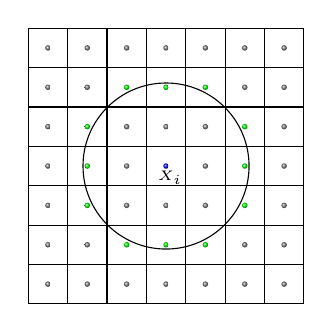
\begin{tikzpicture}
\shade[ball color = blue] (2,2) circle(1pt);
\shade[ball color = green] (1,1.5) circle(1pt);
\shade[ball color = green] (1,2.0) circle(1pt);
\shade[ball color = green] (1,2.5) circle(1pt);
\shade[ball color = green] (3,1.5) circle(1pt);
\shade[ball color = green] (3,2.0) circle(1pt);
\shade[ball color = green] (3,2.5) circle(1pt);
\shade[ball color = green] (1.5,1) circle(1pt);
\shade[ball color = green] (2.0,1) circle(1pt);
\shade[ball color = green] (2.5,1.) circle(1pt);
\shade[ball color = green] (1.5,3) circle(1pt);
\shade[ball color = green] (2.0,3) circle(1pt);
\shade[ball color = green] (2.5,3) circle(1pt);
 \foreach \x in {0.5,3.5}
 \foreach \y in {0.5,1,1.5,2,2.5,3,3.5}
 \shade[ball color = gray](\x,\y) circle (1pt);
 \foreach \x in {1,1.5,2,2.5,3}
 \foreach \y in {0.5,3.5}
 \shade[ball color = gray](\x,\y) circle (1pt);
 \foreach \x in {1.5,2,2.5}
 \foreach \y in {1.5,2.5}
 \shade[ball color = gray](\x,\y) circle (1pt);
 \foreach \x in {1,3}
 \foreach \y in {1,3}
 \shade[ball color = gray](\x,\y) circle (1pt);
 \shade[ball color = gray](1.5,2) circle (1pt);
 \shade[ball color = gray](2.5,2) circle (1pt);
 \foreach \x in {0.5,1,1.5,2,2.5,3,3.5,4.0}
 \draw(\x-0.25,0.25) -- (\x-0.25,4-0.25);
 \foreach \x in {0.5,1,1.5,2,2.5,3,3.5,4.0}
 \draw(0.25,\x-0.25) -- (4-0.25,\x-0.25);
 \draw(2,2) circle(30pt);
\node at (2.05,1.85) {\tiny{$X_i$}};
\end{tikzpicture}
\caption{Discrete mesh node $X_i$ on the equidistant grid and its interaction zone $B_\delta(X_i):=\lbrace X_j \vert \,\vert\vert X_j-X_i\vert\vert \leq \delta\rbrace$. }
\label{fig:emu}
\end{figure}

%----------------------------------------------------------------------------------------
\section{Algorithm}
%----------------------------------------------------------------------------------------

%----------------------------------------------------------------------------------------
\chapter{One-dimensional heat equation}
%----------------------------------------------------------------------------------------



\newpage
\theendnotes